% !TeX spellcheck = en_US
\chapter{Core mass retention}

While this thesis focuses on the water retention after the collisions, the same methods can be applied to the fraction of basalt from the core of the two bodies that remains after the collision. Using the same parameters for interpolation and a separately trained model with the same parameters results in similar results as for water retention. When plotted just like before in Figure \ref{fig:mass_results}, one can see that the results are quite similar. The main difference is that on average there is a slightly higher core mass retention, which can be explained by the fact that weaker collisions might be strong enough to throw the outer water layer into space, but keep the core intact. In addition, it seems like the border between high and low core mass retention is smaller.\todo{better phrase}

When applying the same comparison as described in Section \ref{sec:comparison} the interpolations seem to have a lower accuracy, but still RBF interpolation gives the best results considering slow speed of griddata.


\begin{table}[h]
	\centering
	\begin{tabular}{rcc}
		& {mean squared error} & {mean error} \\
		neural network &        0.043         &    0.167     \\
		RBF &        0.032         &    0.149     \\
		griddata &        0.041         &   0.169
	\end{tabular}
	\caption{prediction accuracy for the different interpolation methods}
	\label{tab:mass_comparison}
\end{table}

\begin{figure}
	\centering
	\begin{subfigure}[t]{0.5\textwidth}
		\centering
		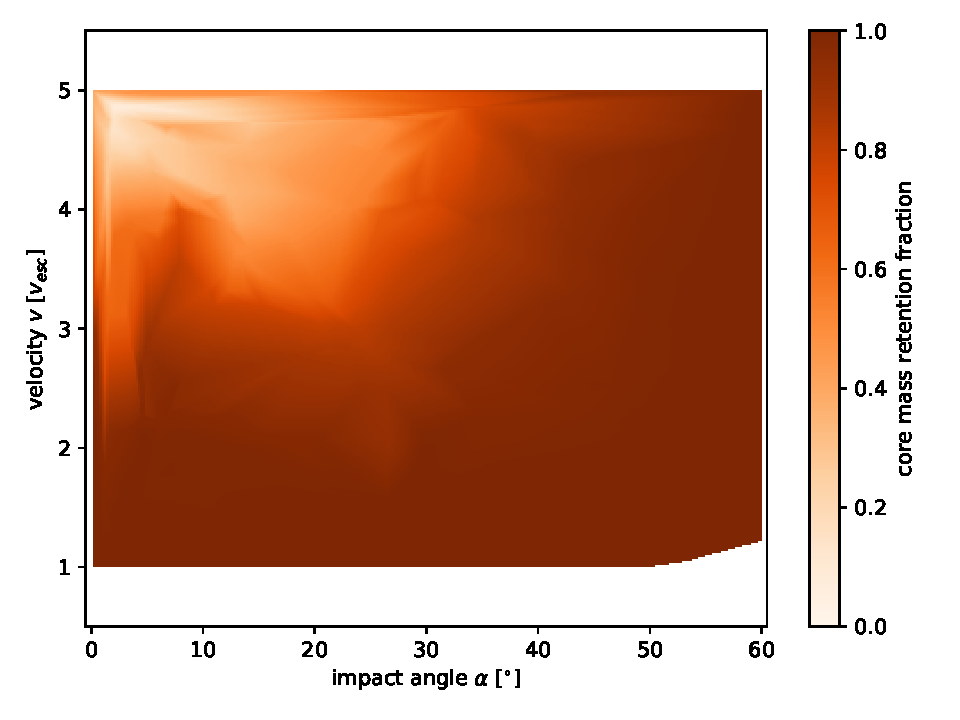
\includegraphics[width=\linewidth]{images/plots/mass_griddata1.pdf}
		\caption{Griddata with $m_{total}=\num{e22}$}
		\label{fig:mass_griddata1}
	\end{subfigure}%
	~ 
	\begin{subfigure}[t]{0.5\textwidth}
		\centering
		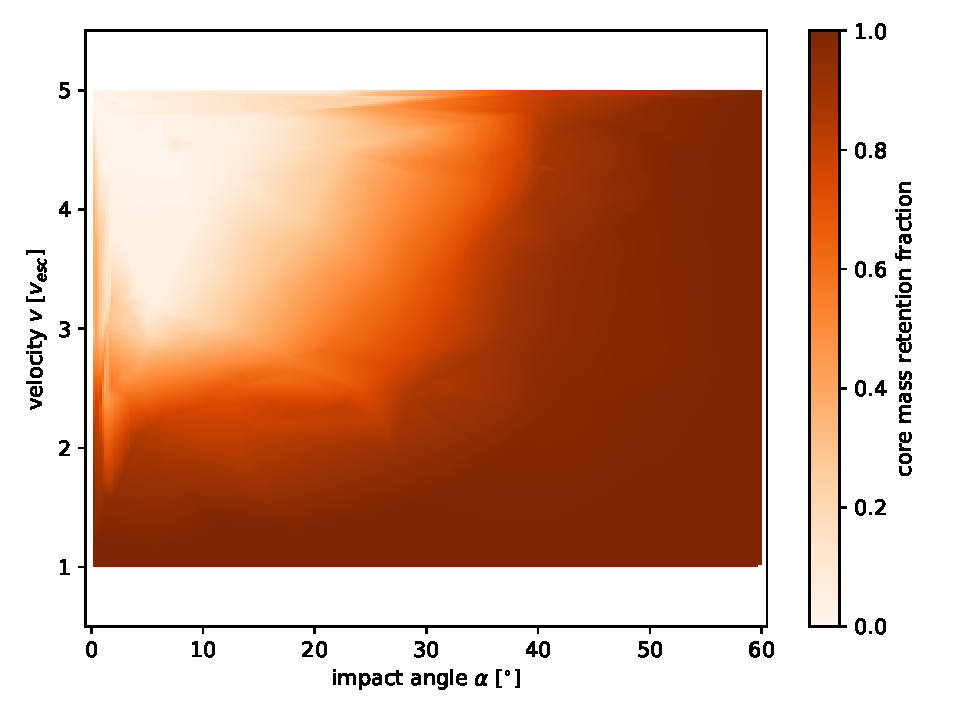
\includegraphics[width=\linewidth]{images/plots/mass_griddata2.pdf}
		\caption{Griddata with $m_{total}=\num{e24}$}
		\label{fig:mass_griddata2}
	\end{subfigure}
~ 
	\begin{subfigure}[t]{0.5\textwidth}
	\centering
	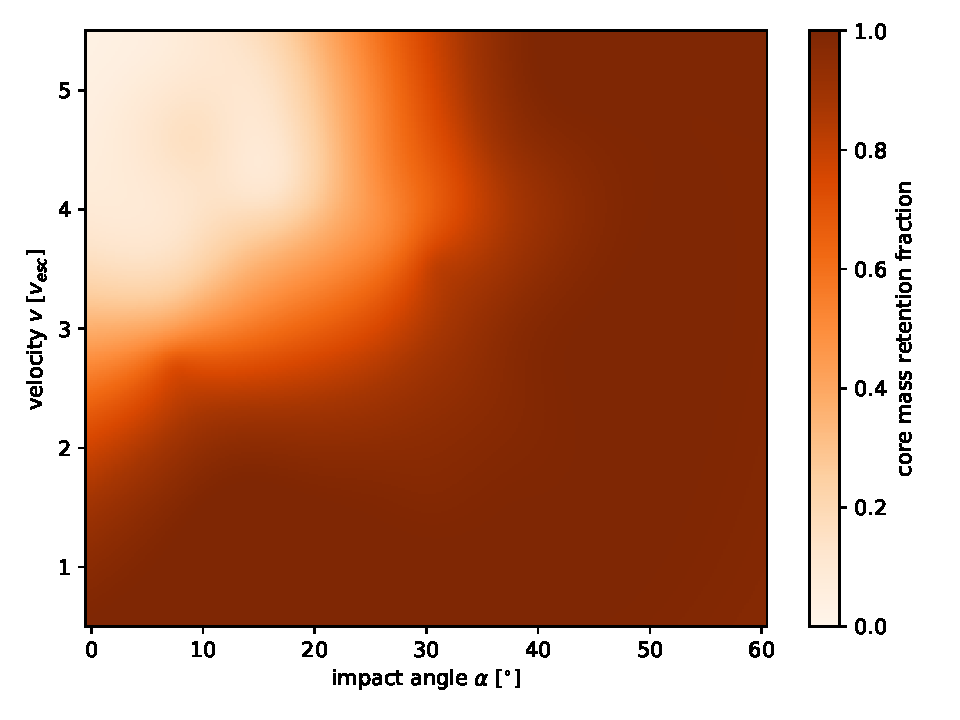
\includegraphics[width=\linewidth]{images/plots/mass_rbf1.pdf}
	\caption{RBF with $m_{total}=\num{e22}$}
	\label{fig:mass_rbf1}
\end{subfigure}%
~ 
\begin{subfigure}[t]{0.5\textwidth}
	\centering
	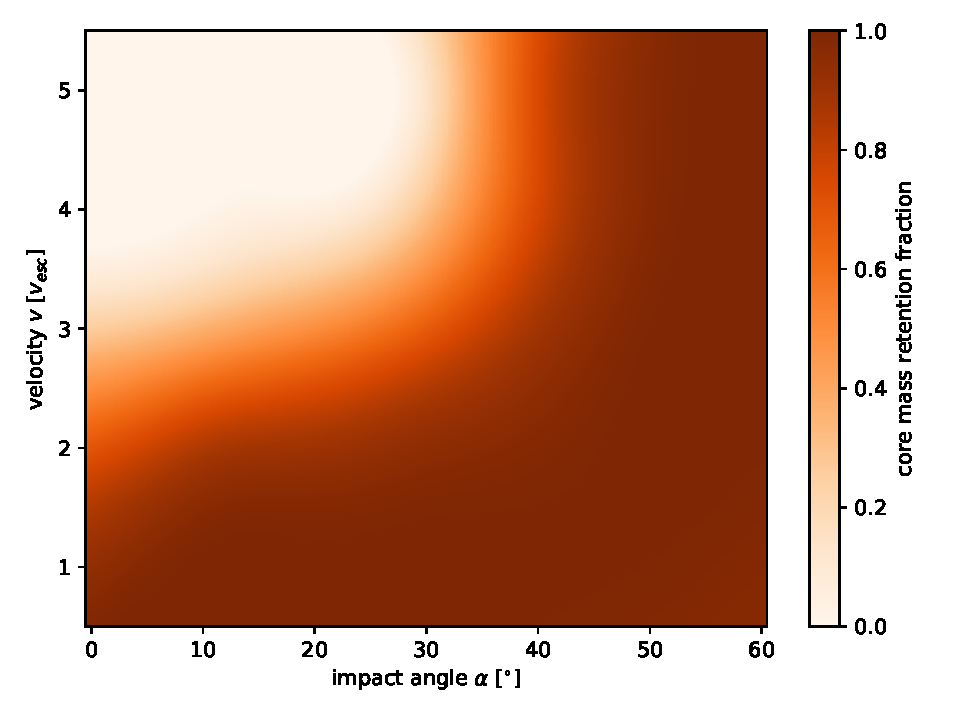
\includegraphics[width=\linewidth]{images/plots/mass_rbf2.pdf}
	\caption{RBF with $m_{total}=\num{e24}$}
	\label{fig:mass_rbf2}
\end{subfigure}
~ 
\begin{subfigure}[t]{0.5\textwidth}
	\centering
	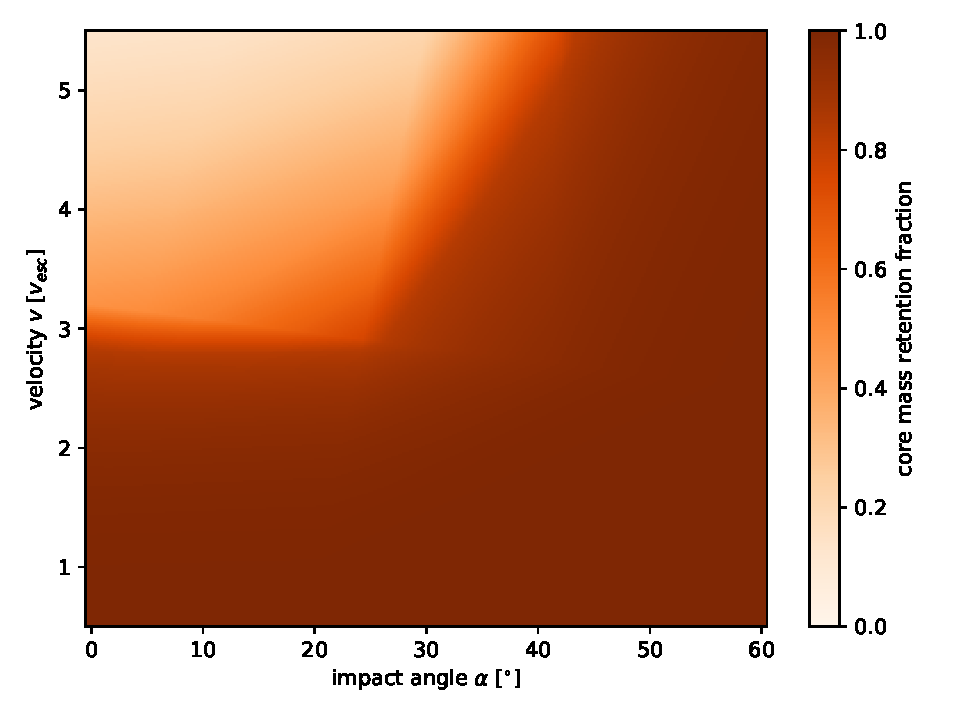
\includegraphics[width=\linewidth]{images/plots/mass_nn1.pdf}
	\caption{Neural Network  with $m_{total}=\num{e22}$}
	\label{fig:mass_nn1}
\end{subfigure}%
~ 
\begin{subfigure}[t]{0.5\textwidth}
	\centering
	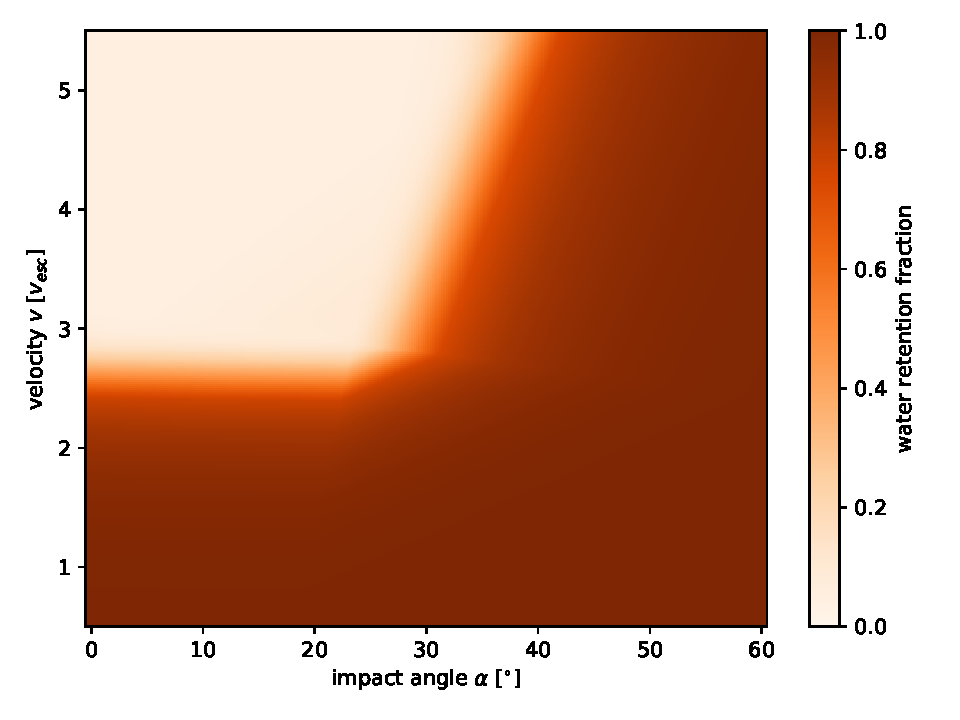
\includegraphics[width=\linewidth]{images/plots/mass_nn2.pdf}
	\caption{Neural Network  with $m_{total}=\num{e24}$}
	\label{fig:mass_nn2}
\end{subfigure}
	\caption{TODO}
	\label{fig:mass_results}
\end{figure}
